\documentclass[journal,12pt,twocolumn]{IEEEtran}
\usepackage{setspace}
\usepackage{gensymb}
\usepackage{xcolor}
\usepackage{caption}
\singlespacing
\usepackage{siunitx}
\usepackage[cmex10]{amsmath}
\usepackage{mathtools}
\usepackage{hyperref}
\usepackage{amsthm}
\usepackage{mathrsfs}
\usepackage{txfonts}
\usepackage{stfloats}
\usepackage{cite}
\usepackage{cases}
\usepackage{subfig}
\usepackage{longtable}
\usepackage{multirow}
\usepackage{enumitem}
\usepackage{mathtools}
\usepackage{listings}
\usepackage{tikz}
\usetikzlibrary{shapes,arrows,positioning}
\usepackage{circuitikz}
\let\vec\mathbf
\DeclareMathOperator*{\Res}{Res}
\renewcommand\thesection{\arabic{section}}
\renewcommand\thesubsection{\thesection.\arabic{subsection}}
\renewcommand\thesubsubsection{\thesubsection.\arabic{subsubsection}}

\renewcommand\thesectiondis{\arabic{section}}
\renewcommand\thesubsectiondis{\thesectiondis.\arabic{subsection}}
\renewcommand\thesubsubsectiondis{\thesubsectiondis.\arabic{subsubsection}}
\hyphenation{op-tical net-works semi-conduc-tor}

\lstset{
language=Python,
frame=single, 
breaklines=true,
columns=fullflexible
}
\begin{document}
\theoremstyle{definition}
\newtheorem{theorem}{Theorem}[section]
\newtheorem{problem}{Problem}
\newtheorem{proposition}{Proposition}[section]
\newtheorem{lemma}{Lemma}[section]
\newtheorem{corollary}[theorem]{Corollary}
\newtheorem{example}{Example}[section]
\newtheorem{definition}{Definition}[section]
\newcommand{\BEQA}{\begin{eqnarray}}
\newcommand{\EEQA}{\end{eqnarray}}
\newcommand{\define}{\stackrel{\triangle}{=}}
\newcommand{\myvec}[1]{\ensuremath{\begin{pmatrix}#1\end{pmatrix}}}
\newcommand{\mydet}[1]{\ensuremath{\begin{vmatrix}#1\end{vmatrix}}}

\bibliographystyle{IEEEtran}
\providecommand{\nCr}[2]{\,^{#1}C_{#2}} % nCr
\providecommand{\nPr}[2]{\,^{#1}P_{#2}} % nPr
\providecommand{\mbf}{\mathbf}
\providecommand{\pr}[1]{\ensuremath{\Pr\left(#1\right)}}
\providecommand{\qfunc}[1]{\ensuremath{Q\left(#1\right)}}
\providecommand{\sbrak}[1]{\ensuremath{{}\left[#1\right]}}
\providecommand{\lsbrak}[1]{\ensuremath{{}\left[#1\right.}}
\providecommand{\rsbrak}[1]{\ensuremath{{}\left.#1\right]}}
\providecommand{\brak}[1]{\ensuremath{\left(#1\right)}}
\providecommand{\lbrak}[1]{\ensuremath{\left(#1\right.}}
\providecommand{\rbrak}[1]{\ensuremath{\left.#1\right)}}
\providecommand{\cbrak}[1]{\ensuremath{\left\{#1\right\}}}
\providecommand{\lcbrak}[1]{\ensuremath{\left\{#1\right.}}
\providecommand{\rcbrak}[1]{\ensuremath{\left.#1\right\}}}
\theoremstyle{remark}
\newtheorem{rem}{Remark}
\newcommand{\sgn}{\mathop{\mathrm{sgn}}}
\newcommand{\rect}{\mathop{\mathrm{rect}}}
\newcommand{\sinc}{\mathop{\mathrm{sinc}}}
\providecommand{\abs}[1]{\left\vert#1\right\vert}
\providecommand{\res}[1]{\Res\displaylimits_{#1}} 
\providecommand{\norm}[1]{\lVert#1\rVert}
\providecommand{\mtx}[1]{\mathbf{#1}}
\providecommand{\mean}[1]{E\left[ #1 \right]}
\providecommand{\fourier}{\overset{\mathcal{F}}{ \rightleftharpoons}}
\providecommand{\ztrans}{\overset{\mathcal{Z}}{ \rightleftharpoons}}
\providecommand{\system}[1]{\overset{\mathcal{#1}}{ \longleftrightarrow}}
\newcommand{\solution}{\noindent \textbf{Solution: }}
\providecommand{\dec}[2]{\ensuremath{\overset{#1}{\underset{#2}{\gtrless}}}}
\makeatletter
\@addtoreset{figure}{problem}
\makeatother
\let\StandardTheFigure\thefigure
\renewcommand{\thefigure}{\theproblem}
\def\putbox#1#2#3{\makebox[0in][l]{\makebox[#1][l]{}\raisebox{\baselineskip}[0in][0in]{\raisebox{#2}[0in][0in]{#3}}}}
     \def\rightbox#1{\makebox[0in][r]{#1}}
     \def\centbox#1{\makebox[0in]{#1}}
     \def\topbox#1{\raisebox{-\baselineskip}[0in][0in]{#1}}
     \def\midbox#1{\raisebox{-0.5\baselineskip}[0in][0in]{#1}}

\vspace{3cm}
\title{\LaTeX Assignment}
\author{Gautam Singh}
\maketitle
\bigskip
\begin{abstract}
This document contains the solution to Exercises 10.4 of the Class 9 NCERT
Mathematics textbook.
\end{abstract}

\problem Two circles of radii 5 cm and 3 cm intersect at two points and the
distance between their centres is 4 cm. Find the length of the common chord.

\solution Let the centres of the two circles be $\myvec{0\\0}$ and 
$\myvec{4\\0}$. The situation is shown in Fig. \eqref{fig:q1}.

\begin{figure}[!ht]
    \centering
    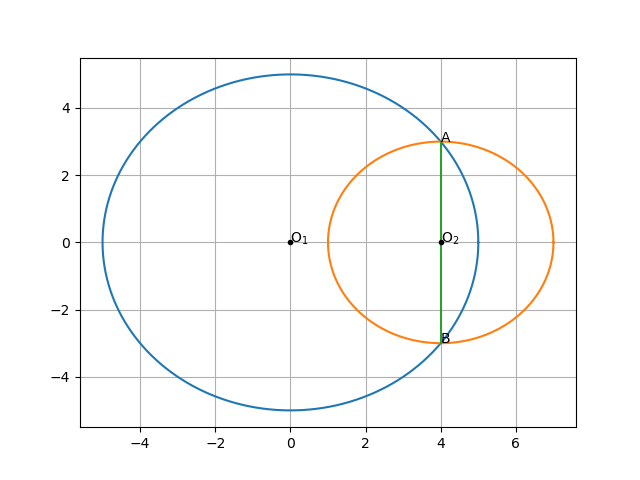
\includegraphics[width=\columnwidth]{figs/10_4_1.png}
    \caption{The common chord in this situation is AB.}
    \label{fig:q1}
\end{figure}

The equations of the circles $O_1$ and $O_2$ are
\begin{align}
    \norm{\vec{x}}^2 - 25 &= 0 \label{eq:q1-1} \\
    \norm{\vec{x}}^2 - 2\myvec{4\\0}^T.\vec{x} + 7 &= 0 \label{eq:q1-2} \\
\end{align}
Substituting \eqref{eq:q1-1} in \eqref{eq:q1-2}, we get
\begin{align}
    \myvec{4\\0}^T.\vec{x} &= 16 \\
    \label{eq:q1-3}
\end{align}
Using \eqref{eq:q1-1}, we see that the intersection points
of the two circles are
\begin{align}
    \vec{x_1} = \myvec{4\\3} \qquad \vec{x_2} = \myvec{4\\-3}
    \label{eq:q1-4}
\end{align}
Thus, the length of the common chord is $\norm{\vec{x_1} - \vec{x_2}} = 6$.

\problem If two equal chords of a circle intersect within the circle, prove 
that the segments of one chord are equal to corresponding segments of the other 
chord.

\solution We know that equal chords of a circle subtend equal angles at the
centre of the circle (see Fig. \eqref{fig:q2}). The area of the minor and major 
segments are (here $\sbrak{.}$ denotes the area of region enclosed by . and 
$\sbrak{O}$ denotes the area of the circle centered at $O$)

\begin{figure}[!ht]
    \centering
    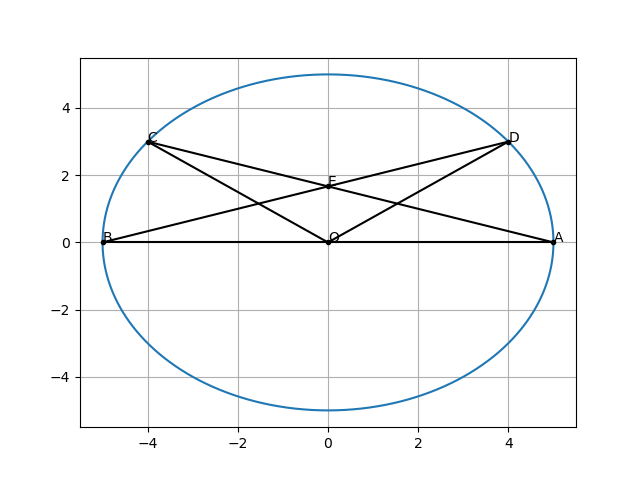
\includegraphics[width=\columnwidth]{figs/10_4_2.png}
    \caption{Two equal chords of a circle create equal segments.}
    \label{fig:q2}
\end{figure}

\begin{align}
    \sbrak{AECDA} &= \sbrak{OCDAO} - \sbrak{OAECO} \\
                  &= \sbrak{OBCDO} - \sbrak{OBEDO} \\
                  &= \sbrak{BEDCB}
    \label{eq:q3-1}
\end{align}
since sectors subtending equal angles at the centre of the circle are of
equal area and equal chords of a circle are equidistant from the centre of the
circle.

Using \eqref{eq:q3-1},
\begin{align}
    \sbrak{AECBA} &= \sbrak{O} - \sbrak{AECDA} \\
                  &= \sbrak{O} - \sbrak{BEDCB} \\
                  &= \sbrak{BEDAB}
    \label{eq:q3-2}
\end{align}
and the conclusion follows.

\problem If two equal chords of a circle intersect within the circle, prove 
that the line joining the point of intersection to the centre makes equal 
angles with the chords.

\solution See Fig. \eqref{fig:q3}. In triangles $OP_1E$ and $OP_2E$,

\begin{figure}[!ht]
    \centering
    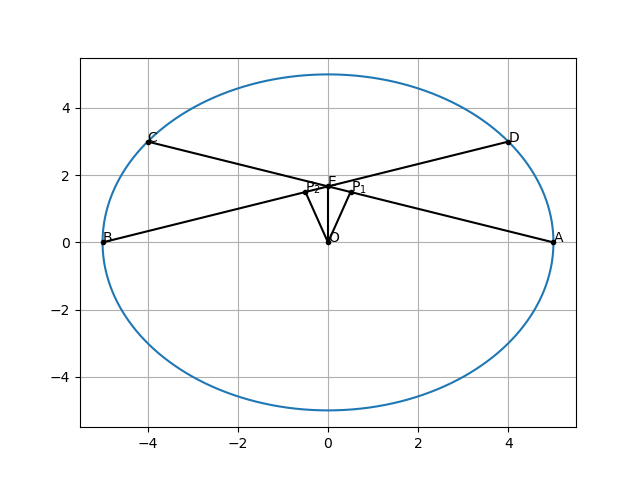
\includegraphics[width=\columnwidth]{figs/10_4_3.png}
    \caption{Equal intersecting chords of a circle make equal angles with $OE$.}
    \label{fig:q3}
\end{figure}

\begin{align}
    \angle{OP_1E} &= \angle{OP_2E} \qquad &\sbrak{\text{Right angles}} \\
    OE &= OE \qquad &\sbrak{\text{Common}} \\
    OP_1 &= OP_2 \qquad &\sbrak{\because AC = BD}
\end{align}
Thus, $\Delta OP_1E \cong \Delta OP_2E$ by RHS criterion. Equating 
corresponding parts, $\angle{AEO} = \angle{P_1EO} = \angle{P_2EO} = \angle{BEO}$
as desired.

\problem If a line intersects two concentric circles (circles with the same 
centre) with centre O at A, B, C and D, prove that AB = CD (see Fig. \eqref{fig:q4}).

\solution We know that the perpendicular dropped from the centre of a circle to a
chord bisects the chord. Therefore, in Fig. \eqref{fig:q4},

\begin{figure}[!ht]
    \centering
    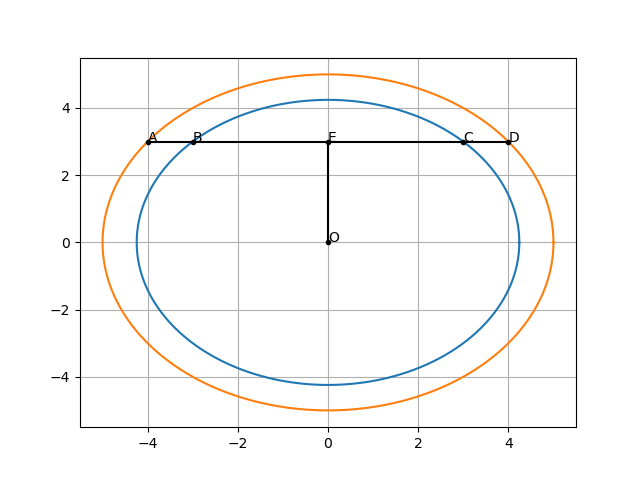
\includegraphics[width=\columnwidth]{figs/10_4_4.png}
    \caption{ABCD intersects the two circles at A, B, C, D. E is the foot of 
    the perpendicular on AD from O.}
    \label{fig:q4}
\end{figure}

\begin{align}
    AE &= ED \\
    BE &= EC \\
    \implies AB = AE - BE &= ED - EC = CD
    \label{eq:q4-1}
\end{align}
as required.

\problem Three girls Reshma, Salma and Mandip are playing a game by standing on 
a circle of radius 5m drawn in a park. Reshma throws a ball to Salma, Salma to 
Mandip, Mandip to Reshma. If the distance between Reshma and Salma and between 
Salma and Mandip is 6m each, what is the distance between Reshma and Mandip?

\solution Suppose that Reshma, Salma and Mandip are located at $R$, $S$ and $M$
as shown in Fig. \eqref{fig:q5}, and have position vectors $\vec{r}, \vec{s} = 
\myvec{5\\0}$ and $\vec{m}$ respectively.

\begin{figure}[!ht]
    \centering
    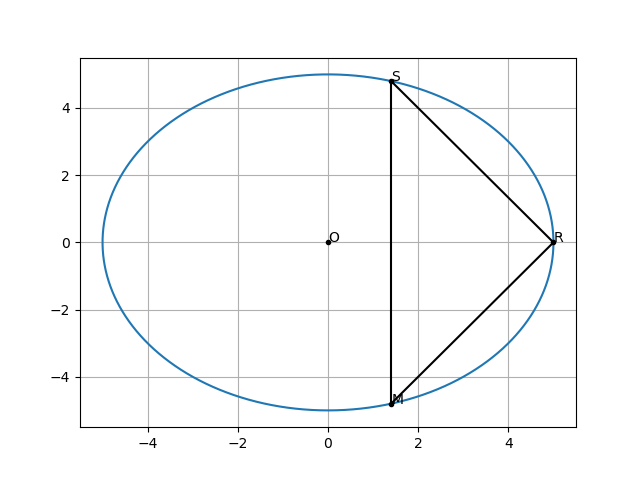
\includegraphics[width=\columnwidth]{figs/10_4_5.png}
    \caption{$RS = SM = 6$}
    \label{fig:q5}
\end{figure}
$\vec{r}$ and $\vec{m}$ satisfy

\begin{align}
    \norm{\vec{x}}^2 &= 25 \label{eq:q5-1} \\
    \norm{\vec{x} - \vec{s}}^2 &= 36 \label{eq:q5-2}
\end{align}

Using \eqref{eq:q5-1} in \eqref{eq:q5-2},
\begin{align}
    \vec{s}^T\vec{x} = 7 
    \label{eq:q5-3}
\end{align}

Using \eqref{eq:q5-3} along with \eqref{eq:q5-1} gives two solutions for $\vec{x}$,
\begin{align}
    \vec{r} = \frac{1}{5}\myvec{7\\24} \qquad \vec{m} = \frac{1}{5}\myvec{7\\-24}
    \label{eq:q5-4}
\end{align}

Thus, the required distance is $\norm{\vec{r} - \vec{m}} = 9.6$m.

\problem A circular park of radius 20m is situated in a colony. Three boys Ankur,
Syed and David are sitting at equal distance on its boundary each having a toy 
telephone in his hands to talk each other. Find the length of the string of each 
phone.

\solution The situation is depicted in Fig. \eqref{fig:q6}.

\begin{figure}[!ht]
    \centering
    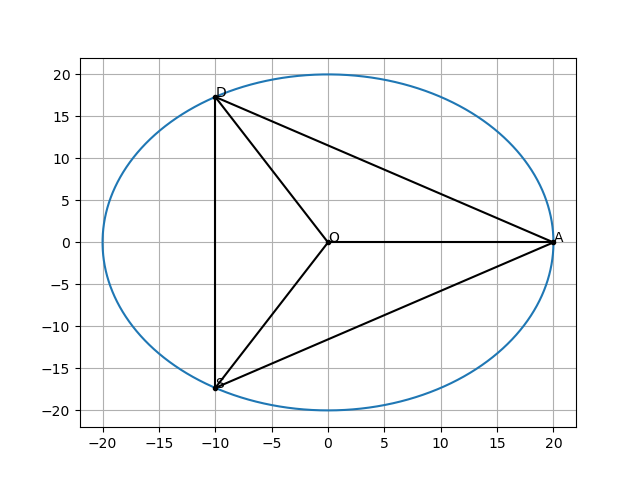
\includegraphics[width=\columnwidth]{figs/10_4_6.png}
    \caption{Triangle ASD is equilateral.}
    \label{fig:q6}
\end{figure}

Suppose the position vectors of Ankur, Syed and David are $\vec{a}, \vec{s}$ 
and $\vec{d}$ respectively. Then,

\begin{align}
    \norm{\vec{a}} = \norm{\vec{s}} = \norm{\vec{d}} = 20 \label{eq:q6-1} \\
    \norm{\vec{a} - \vec{s}} = \norm{\vec{s} - \vec{d}} = \norm{\vec{d} - \vec{a}} \label{eq:q6-2} \\
\end{align}
From \eqref{eq:q6-2}, we get

\begin{align}
    \vec{a}^T\vec{d} = \vec{d}^T\vec{s} = \vec{s}^T\vec{a} \\
    \implies \angle{AOD} = \angle{DOS} = \angle{AOS} = \frac{2\pi}{3}
    \label{eq:q6-3}
\end{align}
Using \eqref{eq:q6-1},

\begin{align}
    \norm{\vec{a} - \vec{d}} &= \sqrt{\norm{\vec{a}}^2 + \norm{\vec{d}}^2 +2\vec{a}^T\vec{d}} \\
    &= \sqrt{400 + 400 + 2\times400\times\frac{-1}{2}} \\
    &= 20\sqrt{3}
    \label{eq:q6-4}
\end{align}
Hence, the required length of the string is $20\sqrt{3}$m.
\end{document}
